% To-Dos:

\chapter{Tap it again, Sam: harmonizing personal environments towards lifelong learning} % Write in your own chapter title

%\begin{quote}
%\textbf{Abstract:} With a focus on the situated support of informal and non-formal
%learning scenarios in ubiquitous learning environments, the presented paper outlines the authors� vision of ambient learning displays � enabling
%learners to view, access, and interact with contextualised digital content
%presented in an ambient way. The vision is based on a detailed exploration of
%the characteristics of ubiquitous learning and a deduction of informational,
%interactional, and instructional aspects to focus on. Towards the vision essential
%research questions and objectives as well as a conceptual framework that
%acquires, channels, and delivers the information framed in the learning process
%are presented. To deliver scientific insights into the authentic learning support
%in informal and non-formal learning situations and to provide suggestions for
%the future design of ambient systems for learning the presented paper concludes with a
%research agenda proposing a research project including a discussion of related
%issues and challenges.
%\end{quote}
\vfill
The increasing number of mobile vendors releasing NFC-enabled devices to the market and their prominent adoption has moved this technology from a niche product to a product with a large market-share. NFC facilitates natural interactions between digital world and physical learning environments. The scaffolding of learning ecologies is a key aspect for lifelong learners in their challenge to integrate learning activities into busy daily life. The contribution of this manuscript is twofold: first, a review of scientific literature in which NFC has been used with a direct or indirect purpose to learn is presented, and potential uses for learners are classified according to their type of interaction; based on these findings the NFC MediaPlayer is presented as an instantiation of an ecology of resources (EoR) in a lifelong learning context. Finally, shortcomings and best practices are highlighted in the conclusions, and future work is discussed.
\vspace{3em}

This chapter is published as: Tabuenca, B., Kalz, M., \& Specht, M. (in press). Tap it again, Sam: harmonizing personal environments towards lifelong learning. International Journal of Advanced Corporate Learning (iJAC)
\clearpage

\section{Introduction}
In a survey by the European Commission time, location and conflicts with other activities have been identified as the core barriers to lifelong learning \cite{EuropeanCommission2007}. Lifelong learners constantly re-design their environments to optimise opportunities interacting with social and other resources towards their learning goals. However, there is little technological support for lifelong learners that typically try to learn in different contexts, are busy with multiple parallel learning tracks, and must align or relate their learning activities to everyday leisure and working activities \cite{Kalz2014}.

On the other hand, visions of ambient intelligence emphasize on the importance in the natural interaction between user and services embedded in the environment or available through mobile devices. \em Natural User Interfaces \em and the \em Internet of Things \em have been predicted to have an impact on education in the short term \cite{Johnson2012}. Tagged objects are widely accepted and the number of connected devices could reach 50 billion by 2020 \cite{Ericsson2011}. Different tagging methods (e.g. visual codes, text recognition, image recognition) allow enriching physical objects with educational resources \cite{Specht2013}. In particular, the prominent adoption of Near Field Communication (NFC) readers in mobile devices has moved this technology from an innovator to an early adopter phase. The NFC Forum\footnote{NFC Forum. Since 2004, this organization develops specifications to ensure interoperability among devices and services. http://nfc-forum.org/} has recently (as of October 2014) estimated that more than 70\% of all smartphones will be equipped with NFC in 2018 (\cite{Bialke2014}).

Lowering the barriers for access to relevant information and support services in frequently used living spaces represents an essential challenge for lifelong learning support. Hence, lifelong learners normally build personal ecologies with the resources available in the environment to support their learning needs. In this scenario, the smartphone plays the role of a hub connecting smart resources coexisting in personal learning environments.

This manuscript aims at gathering previous work in which NFC technology has a potential for learning. This collection aims at inspiring scaffolds to create ecologies of resources in personal learning environments. The document is distributed as follows. Section 2 reviews scientific literature in the field of NFC with a special focus on empirical research. Previous work is classified based on the type of NFC interaction implemented. Taking into account lessons learned in the literature review, section 3 presents a NFC ecology comprising different resources in a frequent learning scenario.
\section{Literature review in NFC technology for learning}
NFC is a radio technology that supports transactions at distances of a few centimetres. NFC standards cover communications protocols and data exchange formats based on existing Radio-Frequency IDentification (RFID) standards. In the current review, we have covered both terms since NFC is an extension to RFID technology. RFID is capable of accepting and transmitting beyond a few meters while NFC is restricted to within four inches.

The underlying search was conducted utilizing the online research repositories of the ScienceDirect, Springer, as well as the IEEE Computer Society. The focus on these repositories is reasonable as they cover a sufficiently large number of relevant publications. Within the Springer digital library an advanced search was performed in December 2014 querying all articles of type journal, proceeding, or transaction that had been published since 2007 (when the first NFC enabled mobile phone was released\footnote{Nokia 6131 NFC phone taps into mobile payment, ticketing and local sharing. , Press. http://bit.ly/1stNFC}) and matching the keywords � \em (NFC learning mobile) OR (RFID learning mobile) \em � as part of the body. The first 100 occurrences ordered by relevance were selected. In a first round, these items were filtered by title and abstract. In a last round, the resulting manuscripts were filtered according to their educational potential. The rest of the repositories were analysed analogously. This review does not aim to be accurate and strict, but rather exploratory to identify suitable learning scenarios and the type of interaction among the resources that better fits the scaffolding of personal learning ecologies with NFC technology.

There are three devices that can be involved in NFC communication: 1) an NFC-enabled mobile device; 2) an NFC external-reader; 3) an NFC tag. NFC mobile phones and NFC external readers can read NFC tags but also other NFC mobile phones working in passive mode. NFC mobile can write NFC tags (Table \ref{tbl:table1}). As a result of this review, previous work is classified (Table \ref{tbl:table2}) according to the type of NFC interaction implemented and best practices are highlighted.

\begin{table}
  \caption{Type of interaction with NFC devices}
  \label{tbl:table1}
  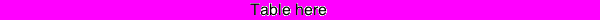
\includegraphics[width=\linewidth]{img/nfcreview_table1}
\end{table}

As a result of this review, scenarios and resources are classified in Table \ref{tbl:table1} according to the type of NFC interaction implemented.

\subsection{Formal Education}
Recent work (\cite{Ebner2013}), envisions some of the potentials NFC technology brings for teaching and learning materials in formal education, with a special focus on connecting digital media and printed learning resources: 1) Distributing learning materials in face-to-face classrooms. Transferring the files from teachers (NFC tag) to students (NFC mobile) avoiding printing on paper and delivering them manually; 2) Enriching printed materials. NFC tags stuck on printed materials facilitate the association of multimedia content; 3) Sharing materials among students. Peer-to-peer communication between mobile devices; 4) Signing delivered practical work and handing it in. For instance, when a student delivers a practical work, the teacher scans the student�s tag with the NFC reader to confirm his/her identity and automatically submits back an email to the student as acknowledgment of reception; 5) Integration with social networks i.e. tap a tag to log in a social network the timestamp in which the arrives to school; 6) Control materials. Teachers can tag the tools in a lab in order to control which resources are assigned to each student; 7) Examinations. NFC tags can be stuck to identity cards from students so teachers can verify their identity in exams.

An introductory course in systems engineering (\cite{Gomez2013}) used hardware components enriched with tags, to provide multimedia resources such as hypertext, audios, videos and animations describing their functionality within the computer. Their experiment concluded with increased learning outcomes for the group of students using this self- paced mobile approach in contrast to the group using the traditional face-to-face lecture.

Similar, \cite{Riekki2013} implemented a pilot study to support children in their efforts in learning to read. Different words written on a poster and a NFC tag attached to them, provided the audio version of the word when the tags were tapped. The results of the pilot study suggested that NFC is a suitable technology for learning to read as a consequence of a positive effect on children�s emergent letter knowledge.
\subsection{Guided tours and fieldtrips}
Excursions of art and museums are typical scenarios where content is delivered based on the parameters supplied by the mobile device. Mobile-guides delivering contextualized audio, video and text, are reviewed in recent work (\cite{Emmanouilidis2013}). This work claims that the current trend is to gradually abandon some of the older localization technologies such as Wi-Fi, infrared and manual user position input. Most of the times, a guide is not necessary because visits to museums are mostly in small groups, and visitors do not want to be overloaded with information. RFID interaction offers a non-intrusive and intuitive interaction in which the user can customize his own learning by approaching the smartphone to a tag attached to a physical object based on his interests on a concrete author, topic, age, etc.

Visitors with limited motivation prefer a broader presentation in contrast to visitors who express an additional interest. \cite{Kuflik2011} implemented different tours and multimedia presentations adapting the content delivered based on the motivation of the visitor. This work concludes the use of RFID as the simplest available technology for accurate customization and positioning inside a building. Previously, \cite{Miyashita2008} had combined RFID tags, and a mobile-PC to use already existing audio guides during a six-month exhibition on Islamic art. Similar, in the work from \cite{Garrido2011} students used NFC enabled phones in the context of a mobile game to know the university campus. Students tapped tags whenever they wanted to communicate to the central game manager their progress within the game and get follow-up assignments. The work from \cite{Sanchez2011a} presents the results of a prototype evaluation that aimed at persuade students to do physical exercise exploring points of interest in the surroundings and tapping them.

Posters can be augmented with different NFC tags to provide a specific feedback based on the tag that is tapped. In the context of a gym in a university campus, Andersen et al. \cite{Andersen2013} created a full size smart-poster with the different muscle groups. When exercising, the user can select a muscle group by tapping that part of the poster so that the information describing training tips for this muscle group is displayed as well as training videos demonstrating some possible exercises.

Interactive panels in public spaces can be used to support social activities. A novel solution (\cite{Tesoriero2014}) based on the concept of collaborative interactive panels facilitates users sharing their opinions and votes about environmental concerns tapping the panels with NFC-enabled mobile devices.

The work from \cite{Tabuenca2014d} on mobile authoring stresses the importance of knowledge and skill acquisition in the same context in which they need to be performed. Hence, the paper pinpoints to NFC tags as a suitable storage for mobile-authored Open Educational Resources (OER) in public spaces as they can be easily dropped, shared or remixed by different users and inspired by the authenticity of learning in context.
\subsection{User identification}
Badges are usually integrated in identification cards to track and locate persons in buildings, floors or rooms with different access policy. Sometimes students cannot access certain resources of a lab outside of a defined schedule or teachers can only access the facilities supplied by their department. Traditional keys are increasingly being supplanted by identification cards that give access to certain places depending on the profile of the user. 

\cite{Sandberg2005} provide a real time unauthorized access alert to clinical staff by integrating instant messaging technology and RFID. If teachers would use this technology, students would be able to locate in which classroom a teacher is giving a lecture. Occasional changes of classroom would be detected by the presence of the teacher in a different classroom, so that a SMS notification would be sent to the students, or displayed on digital boards. Analogously, this technology can be used by parents/teachers to have a real-time account on when do their children/students go to class.

NFC tags are increasingly embedded into wearables like key-rings, bands, clocks, collars, or bracelets. Theses tags can be read through material such as wallets and clothing. The GerAmi system (\cite{Corchado2008}) provides insights on how this technology can be successfully applied in wearables. The objectives of this system are to monitor patients and manage the work of the doctors and nurses. The system is configured with ID-readers above each door in rooms and elevators in the facility. Nurses and Alzheimer patients wear a bracelet containing an RFID chip. Additionally, nurses are equipped with PDAs in order to follow the information, set controllable alarms and locks. Additionally, these hospitals provide wireless access points.

In \cite{Andersen2013} key locations at the campus like caf�s, lecture halls and meeting points, are tagged with NFC tags to check-in when entering these locations. This action is registered in a social network (Foursquare. a social networking layer that enabled a user to share their location with friends, via the "check in" - a user would manually tell the application when they were at a particular location. \footnote{https://foursquare.com}) so friends are aware when a person arrives and to a location i.e. for coffee breaks.

A smart classroom system integrates NFC technology to automate attendance management, locate students, and provide real-time feedback via personal response systems (\cite{Shen2014}).
\subsection{Activity Recognition \& Life Logging}
The work from \cite{Yang2011a} uses RFID technology to identify which activity the user is doing. The operations in their activity theory consider three arguments: \em object, location, and time \em. \em Object \em refers to tangible things that humans can interact with (e.g. dishwasher, fridge, microwave). \em Location \em represents the environmental information where an operation occurs. \em Time \em is the duration over which an operation was conducted. This information can be later analysed to identify behavioural patterns.

The work from \cite{Castro2014} explores behavioural data gathering for assessing functional status and health of older adults using NFC enabled mobile phones.  Participants were provided with a deck of twenty NFC-cards depicting some of their most common activities such as going to the supermarket, cooking, watching TV, or going to the doctor. Finally, they were also given a booklet to jot down the time in which the activities were carried out. The mobile devices were carried around older adults� waists.

More recently, \cite{Curiel2013} propose a platform that activates the most used services on mobile devices, such as making a call, by interacting with NFC tags. Thus, depending on the combination of tags users read, the system will recognize the service to activate (read email, send email, telephone call, see photos, show weather forecast, see news and share information) and the parameters needed for its execution (news source, contact email, phone number).

The NFC LearnTracker (\cite{TabuencaLT2014b}) is a tool for self-regulated learning that facilitates the introspection of learning patterns via analytics. This tool is built assuming that commonly used learning materials are tagged with NFC tags. The student taps the tag every time he starts and stops learning, these timestamps are recorded, and the activities can be later analysed with chart visualizations upon their duration, time of the day or used resource.
\subsection{Smart home}
There is an increasing number of publications in the field of smart home. The work from \cite{Sadri2011} surveys ambient intelligence and its application in different contexts, in particular, embedding NFC tags in different.  The GENIO project \cite{Garate2005} presented a fridge that keeps track of the (RFID tagged) goods consumed by the user. Similar, \cite{Reitberger2014} uses visualizations to provide feedback on food consumption clustering the nutrients by categories.

The work from Tran \& Mynatt (\cite{Tran2003,Tran2004}) presents a pilot where a mirror enriched with RFID records repeated frequent tasks (e.g. \em �Has anyone fed the fish?�, �Did I take my medication an hour ago, or did I decide to wait a bit longer?� \em) for which memory-confusion could arise. This system is presented as a long-term memory system for activities that are repeated often and are not part of a strict routine.
\subsection{Support of disabled people}
This section gathers cases in which NFC technology facilitates learning for people with disabilities. The article from \cite{Ivanov2014} presents a mobile service that enables blind-environment interaction through voice-augmented objects by tagging objects with an associated voice-based description. Users can both drop their voice recording in a tag or listen already existing ones. Blind users can later use the service to scan surrounding augmented objects and verbalize their identity and characteristics. \cite{Jafri2014} proposes a solution for teaching Braille letter-recognition to young blind children manipulating NFC-tag embedded blocks with Braille letters embossed on their sides. Braille letter recognition is taught and reinforced through various exercises and games and auditory feedback is provided via a speech interface from a computer attached to the NFC readers.
\subsection{Payment systems and simulations}
The coffee card application is a combination of a prepaid service and loyalty card \cite{Andersen2013} implemented in a campus. Students can recharge 11 cups of coffee for the price of 8 so the prepaid coffee cups are stored on the NFC card. Each time a coffee is bought, the student taps the NFC reader connected to a tablet computer that records the payment. This system could be used to implement serious games to simulating money, transactions, badges or roles in schools.  Indeed, RFID technology has been previously experimented supporting the simulation of roles and scenarios on interactive tables (\cite{Kubicki2011}). As result of this experience, the authors highlight RFID as an interesting approach as they allow the storage of information directly within the tangible objects.
\subsection{Logistics \& object identification}
The ten-year academic review conducted by \cite{Ngai2008} reveals the increasing importance of this technology in the field of logistics. As a consequence of this review, the authors highlight RFID technology as a hot topic in the field of retailing, library services, animal detection, food, and supply chain management. More specific, the work from \cite{Ting2011} reviews the use of RFID in medical organizations for the purpose of managing and tracking medical equipment, monitoring and identifying patients, ensuring that the right medication is given to the right patient, and preventing the use of counterfeit medicine. Additionally, the author presents an exploratory case study conducted in a medical organization offering valuable insight on the use of RFID in medical organizations. The work from \cite{Bacheldor2006} describes an implementation on how to locate medical assets by using an RFID-based real-time location system.
\subsection{Results of the review}
The results of the review envision a trend in which mobile devices are mostly used for reading tags in the last years in contrast to early years where fixed static external readers where used to decode tag. Table \ref{tbl:table2} shows that mobile-to-mobile NFC transfer does not seem to be a frequently implemented practice yet. On the other hand, the most common implementation is the enrichment of tangible objects with NFC tags to be later interpreted as a command by a mobile device. These command are normally associated with third party resources that trigger a subsequent action like inserting data on a database, providing feedback, a description of the object that is tapped or sharing the action in social networks. Additionally, we can observe that mobile devices are mostly used for reading other tags, but not yet commonly used for dropping (writing) information on them.
\begin{table}
  \caption{Classification of ecologies by type of NFC interaction}
  \label{tbl:table2}
  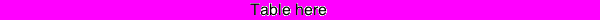
\includegraphics[width=\linewidth]{img/nfcreview_table2}
\end{table}
\section{A seamless learning ecology for video casting}
In the literature review we have presented different ways on how NFC technology can facilitate seamless interactions in different contexts. Harmonizing personal learning environments is key to enable smooth access to learning contents, in particular, with natural interactions and suitable visualizations.

Videos are nowadays a big proportion of the learning materials provided in online courses, i.e. in Learning Management Systems (LMS) or Massive Open Online Courses (MOOCs). Most of the times, these videos are released to be downloaded from a learning management system, or, publicly shared to be remotely visualized from repositories (i.e. YouTube, vimeo). Starting a learning activity in an online course normally requires the user to switch-on the device (or unlock), open a browser, login the platform, navigate to look for the desired resource, and finally display the video. This approach presents the following barriers for seamless access to video content:
\begin{enumerate}
\item Time. Sometimes reaching the learning content might require more time than watching the video itself (i.e. booting a computer). Access to learning content should be guaranteed in the least time possible in order to facilitate the embedment of learning activities in spontaneous scattered moments along the day (i.e. waiting times, commercial breaks).
\item Interaction. Reaching the learning content in LMSs or MOOCs requires multiple clicks. Access to learning content should be accomplished in the least number of clicks possible otherwise the student would not bother to start a learning activity.
\item Visualization. The screens from mobile devices, tablets, or even laptops are not big enough to display videos. Videos should be streamed with a quality that guarantees the user can smoothly accomplish objectives of the learning resource with the least visual overload.
\end{enumerate}
Herby, we present the NFC Media Player, an ecology of resources (\cite{Luckin2008}) that aims at lowering these barriers inspired on the work presented in the literature review.

\subsection{The NFC MediaPlayer}
This section describes the NFC MediaPlayer, an Ecology of Resources (EoR) \cite{Luckin2010} in which the learner is encouraged to explore forms of available assistance in the environment. The EoR is a learner-centric approach comprising three layers (see figure \ref{fig:1}a): 1) the \em Zone of Proximal Development (ZPD) \em ; 2) the \em Zone of Proximal Adjustment (ZPA) \em ; the \em Zone of Available Assistance (ZAA) \em . 
\begin{figure}
     
\includegraphics[width=1\linewidth]{img/nfcreview_fig1}
     \caption{Ecology of resources}
     \label{fig:1}
\end{figure}
ZPD represents what the user can learn by himself with his potential ability and the interactions that can arise from previous experiences. Lifelong learners are intrinsically motivated to learn and to re-design their context with the aim to optimise opportunities for interactions with social and other resources capable of assisting learners perform towards their objectives (design of ZPA (\cite{Vygotsky1978})). Here is where the figure of the \em More Able Partner (MAP) \em represented by the mobile device plays a key role as the main supporter for lifelong learners. Recognising the role of the MAP is fundamental to lifelong learners since they are able to identify potential types of assistance to the learner. Likewise, the relationship between User and MAP supports the progression from ZAA to ZPA. The ZAA is described as the variety of resources within the learner's world that could provide different qualities and quantities of assistance, and that might be available to the learner at a particular point of time. 

For the specific case implemented in this manuscript, NFC technology facilitates the scaffolding of learning activities bringing resources closer to the user supported by a mobile device. E.g. a user can use his/her mobile device to watch a multimedia video stored in a remote repository (ZAA) by taping with the mobile device (MAP) on a NFC tag that is bound to the content (ZPA). Figure \ref{fig:1}b illustrates the resources comprised in this model. Lifelong learners scaffold personal learning ecologies using them as follows:
\paragraph{Environment}
This resource refers to the locations where the lifelong learner is normally used to learn. A recent survey to lifelong learners on mobile usage habits for learning (\cite{Tabuenca2013}) reveals that there is an association between the type of learning activity being performed (read, write, listen, watch) and the concrete location where it takes place. More specifically, at the living room and sitting in the sofa was reported as the most suitable environment to watch videos using their mobile devices for learning purposes. The NFC MediaPlayer ecology has been implemented to provide seamless support for learning in this specific environment.
\paragraph{Knowledge}
This resource refers to the subject, skills or anything that the user wants to learn. In this case, the NFC MediaPlayer is illustrated with the case of a user interested to acquire knowledge on the topic �technology-enhanced learning�.
\paragraph{Tools}
This resource refers to the tools that the lifelong learner uses to learn. The NFC MediaPlayer comprises the following tools that are further described in the following section: HDMI display; digital media player; 5 NFC tags; NFC-enabled smartphone. 
\paragraph{Filters}
Luckin [39] defines filters as the constraints or restrictions that learner find to manage the \em environment \em, use \em tools \em, or acquire \em knowledge \em. In this manuscript, the filters for the NFC MediaPlayer are aligned with the three barriers enumerated above: 1) time; 2) interaction; 3) visualization.
\begin{figure}
     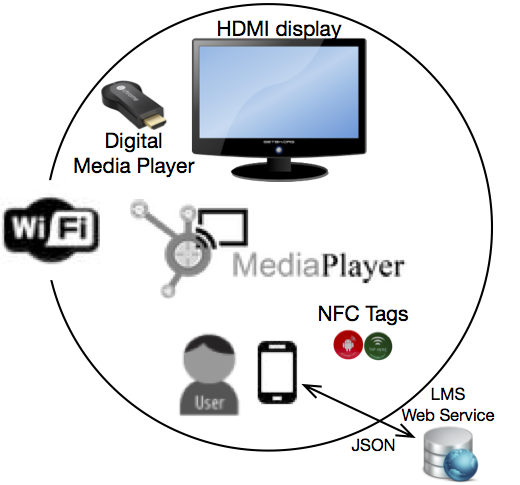
\includegraphics[width=1\linewidth]{img/nfcreview_fig2}
     \caption{NFC MediaPlayer�s ecology of resources}
     \label{fig:2}
\end{figure}
\subsubsection{Implementation}
The NFC MediaPlayer has been released in January 2015 as part of a larger research aiming to provide ubiquitous support for lifelong learning with mobile technology. The source code of this tool is available\footnote{NFC MediaPlayer open source code repository: https://code.google.com/p/lifelong-learning-hub/source/checkout?repo=mediaplayer} under an open license\footnote{Licensed under the Apache License, Version 2.0. http://www.apache.org/licenses/LICENSE-2.0} to facilitate customization and extension to further learning environments, communities, etc. 

This section describes the tools that conform the ecology (See figure \ref{fig:2}):
\paragraph{Digital media player}
In the very last months, WI-FI enabled digital media players have arrived to the market: Google Chromecast\footnote{Google Chromecast. http://www.google.com/intl/en/chrome/devices/chromecast/} (July 2013), Roku\footnote{Roku streaming stick. http://www.roku.com/products/streaming-stick} (March 2013); Apple TV\footnote{Apple TV streamcater http://www.apple.com/appletv/} (January 2013). These devices broadcast audio and video content on a High-Definition display by direct streaming via WI-FI from the Internet. These devices stream multimedia content based on the commands (Play, Pause \& Stop) triggered from another networked device (i.e. laptop, tablet, mobile). The basic operation is that using your personal device as a remote and selecting the desired multimedia, the content is automatically broadcasted in the HDMI display where the digital media player is plugged. The ecology presented in this manuscript has been developed for Google Chromecast\footnote{Google Cast SDK. https://developers.google.com/cast/docs/reference/}.
\begin{figure}
     
\includegraphics[width=1\linewidth]{img/nfcreview_fig3}
     \caption{NFC MediaPlayer. JSON file playlist}
     \label{fig:3}
\end{figure}
\paragraph{HDMI displays}
HDMI displays facilitate the visualization of videos independently of the dimension for which they were designed. When streaming video from the digital media player, the audio volume is controlled from the remote of the HDMI display and not from the client device (mobile device, tablet or laptop). This feature makes the interaction much more natural and integrated within daily life environment.
\paragraph{NFC enabled smartphone}
The mobile phone plays the role of a remote communicating with all the previous elements in the ecology. A NFC-enabled smartphone is able to decode the command recorded in the tag (NDEF message), and trigger the action pre-mapped for that action. 
\paragraph{NFC MediaPlayer app}
The NFC MediaPlayer app has been developed and released\footnote{NFC MediaPlayer in Google Play. https://play.google.com/store/apps/details?id=org.ounl.lifelonglearninghub.mediaplayer} for Android mobile phones in January 2015 (Beta version). When the app starts, the JSON file (Figure \ref{fig:3}) containing the information describing the list of videos to be presented in the playlist, namely, title, subtitle, author, thumbnail images, and the URL where the video is stored, is requested to a remote webservice. 
\begin{figure}
     
\includegraphics[width=1\linewidth]{img/nfcreview_fig4}
     \caption{NFC MediaPlayer�s playlist}
     \label{fig:4}
\end{figure}
The interface navigation within the app has two screens:
\begin{enumerate}
\item Playlist screen (See Figure \ref{fig:4}b). The home screen of the app. Lists the information describing the videos that can be streamcasted. When a video in the list is clicked, the cast screen with the selected video is displayed.
\item Cast screen (Figure \ref{fig:5}b). Displays the information of the video selected in the list. The video starts when the play button starts or stops when in the pause button is clicked. The video can be moved forward or backward using the slider. The video is streamcasted to the HDMI Display depending on whether the Chromecast icon on the top right corner is selected or not.
\end{enumerate}
\begin{figure}
     
\includegraphics[width=1\linewidth]{img/nfcreview_fig5}
     \caption{NFC MediaPlayer�s casting}
     \label{fig:5}
\end{figure}
\paragraph{Programmable NFC Tags}
This ecology includes five tags configured to trigger the following actions:
\begin{itemize}
\item Positioning. The 1)\em positioning \em tag is configured to work in the playlist screen (Figure \ref{fig:4}b). When this tag is tapped (middle bottom tag in the whiteboard on figure \ref{fig:4}a/\ref{fig:5}a), the focus advances in the playlist marking in orange colour the active item.
\item Video casting. The 2)\em play \em and 3)\em pause \em tags are configured to work in the cast screen (Figure \ref{fig:5}b). When the play tag is tapped (left middle tag in the whiteboard on figure \ref{fig:4}a/\ref{fig:5}a), the active video is streamcasted to the HDMI display. The video is paused when the pause tag (right middle tag in the whiteboard) is tapped.
\item Navigation. The 4)\em playlist \em and 5)\em cast \em tags are configured to navigate between the playlist screen (figure \ref{fig:4}b) and the cast screen (Figure \ref{fig:5}b). When the playlist tag is tapped (left top tag in the whiteboard) the app presents the playlist screen. When the cast tag is tapped (right top tag in the whiteboard) the app presents the cast screen.
\end{itemize}
\section{Discussion and Conclusions}
This manuscript proposes the use of NFC technology towards the harmonization between digital and physical worlds for learning.

The literature review presents daily life scenarios (formal education settings, workplaces, museums, guided tours, fieldtrips, life-logging, smart home, simulations, logistics) where NFC technology has been previously used. Findings in the literature review reveal the increasing use of NFC-mobile devices for reading tags, in contrast to external reader. This fact is probably strengthen by the proliferation of NFC-enabled mobile devices and the increasing adoption of NFC technology in the last years (\cite{Bialke2014}). The review shows that using mobile devices to drop (write content) on tags is not a developed practice yet in contrast to reading content that is the most popular use. 

On the other hand, this manuscript highlights the potential of NFC technology to facilitate the scaffolding of personal learning environments binding learning activities to daily physical spaces. The \em NFC MediaPlayer \em is presented as a real instantiation of ecology of resources in a frequent lifelong learning environment tackling three barriers:
\begin{enumerate}
\item Time. Reducing the time to start a learning activity.
\item Interaction. Reducing the number of clicks to access the learning content to zero clicks.
\item Visualization. Streamcasting video learning contents in a High-Definition quality in contrast to small-sized screens like mobiles, tablet or laptops.
\end{enumerate}
This ecology increases the chances of learning in scattered moments (i.e. waiting times, commercial break on TV) replacing this perceived "lost time� into perceived "productive time". 

In future research, we will scaffold ecologies to provide effective feedback services for learning (i.e. ambient displays, recommendations, analytics) and to foster meta-cognitive skills (\cite{Tabuenca2014}). 






